\chapter{Problém maximálníhu řezu}

\section{Formulace úlohy}

Mějme neorientovaný graf $G = (V, E)$ s nezáporným ohodnocením hran $w$. Cílem je rozložit množinu vrcholů $V$ na nejvýše $k \in \mathbf{N} \setminus \left\{ 1 \right\}$ disjunktních množin tak, aby součet hran spojující různé množiny byl maximální. Pokud $k = 2$ hovoříme o úloze \textbf{MAX CUT} a pro $k \geq 3$ o úloze \textbf{MAX $k$-CUT}.

\section{Úloha MAX CUT}

Nejprve se podíváme na aproximační algoritmus z článku \textbf{[REF]} pro úlohu MAX CUT.

\subsection*{Striktní kvadratický program pro MAX CUT}

\textbf{Kvadratický program} je problém maximalizace / minimalizace kvadratické funkce celočíselných proměnných, vzhledem ke kvadratickým omezením těchto proměnných. Je-li navíc každý monom (jednočlen) cenové funkce i daných omezení stupně $0$ nebo $2$, potom mluvíme o \textbf{striktním kvadratickém programu}.

Dále odvodíme striktní kvadratický program pro úlohu MAX CUT. Nechť $y_i \in \left\{ 1, -1 \right\}$ je proměnná příslušná vrcholu $i$. Množiny $S$ a $\bar{S}$ definujeme následovně
$$
    S = \left\{ i \in V \mid y_i = 1 \right\}, \bar{S} = \left\{ i \in V \mid y_i = -1 \right\}.
$$
Pokud $i \in S$ a $j \in \bar{S}$, potom je součin $y_i y_j = -1$ a chceme, aby tato hrana přispívala hodnotou $w_{ij}$ k cenové funkci. Ve zbylých dvou možnostech je $y_i y_j = 1$ a chceme, aby se hodnota cenové funce nezměnila. Použitím těchto podmínek definujeme striktní kvadratický program.

\begin{equation}\tag{SQ-MAX-CUT}
    \begin{split}
        OPT = &\max \frac{1}{2} \sum_{1 \leq i < j \leq n} w_{ij} (1 - y_i y_j) \\
        &\forall i \in V:\ y_i^2 = 1, \\
        &\forall i \in V:\ y_i \in \mathbf{Z}.
    \end{split}
    \label{eq:SQ-MAX-CUT}
\end{equation}


\subsection*{Vektorový program pro MAX CUT}

Poznamenejme jen, že úloha celočíselného programování je NP-těžká. Proto se dále budeme zabývat relaxací úlohy~\ref{eq:SQ-MAX-CUT}, což znamená, že upustíme od podmínek celočíselnosti a původní úlohu relaxujeme vektorovým programem. Modifikujeme tedy program~\ref{eq:SQ-MAX-CUT} tak, že každý součin $y_i y_j$ nahradíme skalárním součinem vektorů $\langle \mathbf{v}_i, \mathbf{v}_j \rangle$ v $\mathbf{R}^n$. Dostáváme následující vektorový program.

\begin{equation}\tag{V-MAX-CUT}
    \begin{split}
        RELAX = &\max \frac{1}{2} \sum_{1 \leq i < j \leq n} w_{ij} (1 - \langle \mathbf{v}_i, \mathbf{v}_j \rangle) \\
        &\forall i \in V:\ \langle \mathbf{v}_i, \mathbf{v}_i \rangle = 1 \\
        &\forall i \in V:\ \mathbf{v}_i \in \mathbf{R}^n
    \end{split}
    \label{eq:V-MAX-CUT}
\end{equation}


\subsection*{Semidefinitní program pro MAX CUT}

Uvedeme si ještě semidefinitní formulaci předchozí vektorové relaxace. Nechť $W$ je matice vah jednotlivých hran taková, že nenulové prvky má pouze nad diagonálou a $w_{ij}$ je váha hrany $ij$. Matice $J$ je matice samých jedniček.

\begin{equation}\tag{SDP-MAX-CUT}
    \begin{split}
        RELAX = &\max \frac{1}{2} W \bullet (J - Y) \\
        &\forall i \in V:\ y_{ii} = 1 \\
        &Y \succeq 0
    \end{split}
    \label{eq:SDP-MAX-CUT}
\end{equation}

\subsection*{Randomizovaný zaokrouhlovací algoritmus}

Mějme dva vektory $\mathbf{a}_i, \mathbf{a}_j$ optimálního řešení programu~\ref{eq:V-MAX-CUT}. Označme $\Theta_{ij}$ úhel, který tyto vektory svírají. Z podmínky
$$
    \forall i \in V:\ \langle \mathbf{v}_i, \mathbf{v}_i \rangle = 1
$$
dostáváme, že $\langle \mathbf{a}_i, \mathbf{a}_j \rangle = \cos \Theta_{ij}$ a příspěvěk těchto vektorů k optimálnímu řešení je
$$
    \frac{w_{ij}}{2} (1 - \cos \Theta_{ij}).
$$
Tedy čím \uv{blíž} je úhel $\Theta_{ij}$ hodnotě $\pi$, tím větší příspěvěk mají tyto vektory k hodnotě optimálního řešení. Dále si uvedeme algoritmus pro řešení úlohy MAX-CUT a jeho analýzu.

\begin{alg}[MAX-CUT]$ $
    \begin{enumerate}
        \item Najdi řešení $\mathbf{a}_1, \dots, \mathbf{a}_n$ programu~\ref{eq:V-MAX-CUT}.
        \item Zvol náhodně vektor $\mathbf{r}$ na jednotkové sféře $S_{n-1}$.
        \item $S = \left\{ i \in V \mid \langle \mathbf{a}_i, \mathbf{r} \rangle \geq 0 \right\}$.
    \end{enumerate}
\end{alg}

Začneme dvěma lemmaty.

\begin{lm}
    Nechť $X_{ij}$ je jev takový, že vrcholy $i$ a $j$ jsou od sebe separovány, tj. jsou v různých množinách. Potom
    $$
        P\left[ X_{ij} \right] = \frac{\Theta_{ij}}{\pi}.
    $$
    \label{lemma:sep}
\end{lm}

\begin{proof}
    Vektory $\mathbf{a}_i, \mathbf{a}_j$ generují rovinu. Uvažme projekci náhodného vektoru $\mathbf{r}$ na jednotkové sféře $S_{n-1}$ do této roviny. Potom vrcholy $i$ a $j$ jsou separovány, jestliže
    $$
        \langle \mathbf{a}_i, \mathbf{a}_j \rangle = \langle \mathbf{r}, \mathbf{a}_i \rangle + \langle \mathbf{r}, \mathbf{a}_j \rangle
    $$
    \begin{center}
        nebo
    \end{center}
    $$
        \langle \mathbf{a}_i, \mathbf{a}_j \rangle = \langle \mathbf{-r}, \mathbf{a}_i \rangle + \langle \mathbf{-r}, \mathbf{a}_j \rangle.
    $$
    Předchozí podmínku separace vrcholů ilustruje obrázek~\ref{fig:lemma_plane}.
\end{proof}

\begin{figure}[h!]
    \centering
    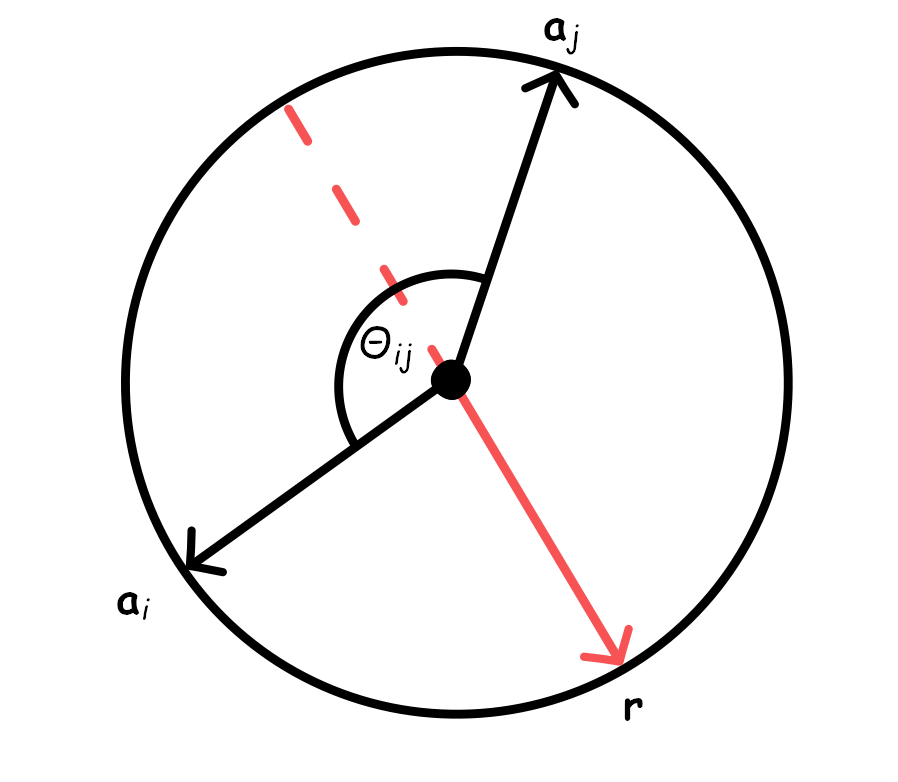
\includegraphics[width=0.5\textwidth]{img/lemma_plane.png}   
    \caption{Separace vrcholů $i$, $j$ náhodným vektorem $\mathbf{r}$.}
    \label{fig:lemma_plane}
\end{figure}


\begin{lm}[KNUTH 2, 135]
    Nechť $\mathbf{x} = (x_1, \dots, x_n)$ je vektor, jehož prvky jsou zvoleny nezávisle z normovaného normální rozdělení $N(0,1)$. Potom $\mathbf{r} = \frac{\mathbf{x}}{\|\mathbf{x}\|_2}$ je náhodný vektor, který leží na jednotkové sféře $S_{n-1}$.
\end{lm}

Dále ukážeme, jak \uv{dobrou} aproximaci algoritmem~\textbf{REF} dostaneme. Označme
$$
    \alpha = \min_{0 \leq \Theta \leq \pi} \frac{2 \Theta}{\pi (1 - \cos \Theta)}.
$$
Snadno se ukáže, použitím derivace, že $\alpha \approx 0.87856$.

\begin{lm}
    Nechť $Y$ je náhodná veličina, která označuje součet vah hran, které vedou z $S$ do $\bar{S}$, nalezeny algoritmem~\textbf{REF}. Potom
    $$
        E\left[ Y \right] \geq \alpha \cdot RELAX.
    $$
\end{lm}

\begin{proof}
    Z definice čísla $\alpha$, pro $0 \leq \Theta \leq \pi$, dostáváme
    \begin{equation}
        \frac{\Theta}{\pi} = \frac{2 \Theta}{\pi (1 - \cos \Theta)} \cdot \frac{1 - \cos \Theta}{2} \geq \frac{\alpha}{2} (1 - \cos \Theta).
        \label{eq:proof_1}
    \end{equation}
    Použitím lemmatu~\ref{lemma:sep} a nerovnosti~\ref{eq:proof_1} dostáváme
    \begin{equation*}
        \begin{split}
            E\left[ Y \right] &= \sum w_{ij} P\left[ X_{ij} \right] \\
                              &= \sum w_{ij} \frac{\Theta_{ij}}{\pi} \\
                              &\geq \frac{\alpha}{2} \sum w_{ij} (1 - \cos \Theta_{ij}) \\
                              &= \alpha \cdot RELAX.
        \end{split}
    \end{equation*}
\end{proof}

Poznamenejme, že samozřejmě platí
$$
    OPT \geq E\left[ Y \right] \geq \alpha \cdot RELAX.
$$

Definujeme \textbf{mezeru celočíselnosti} relaxace (pro maximalizační problém) jako
$$
    \inf_{I} \frac{OPT(I)}{RELAX(I)},
$$
kde infimum probíhá přes všechny instance $I$ daného programu. Tedy mezera celočíselnosti relaxace~\ref{eq:V-MAX-CUT} je alespoň $\alpha \approx 0.87856$.

Předchozí odvození je založeno na střední hodnotě náhodné veličiny $Y$. Proto kroky \textbf{2} a \textbf{3}, v algoritmu, opakujeme vícekrát a jako výsledek zvolíme množinu $S$, která dává největší součet hran z $S$ do $\bar{S}$. Dále jen specifikujeme kolikrát musíme tyto kroky opakovat. Kompletní důkaz je v \textbf{CITE}. Zvolíme tedy $\varepsilon > 0$ (malé), nechť
$$
    c = \frac{\varepsilon \alpha}{2 + 2\varepsilon - \alpha},
$$
a kroky \textbf{2}, \textbf{3} opakujeme $\lceil \frac{1}{c} \rceil$-krát.


\section{Úloha MAX $k$-CUT}

V následující části si uvedeme jen formulace několika programů pro úlohu MAX-$k$-CUT.

\subsection*{Frieze-Jerrum a MAX-$k$-CUT}

\begin{equation}\tag{FJ-MAX-$k$-CUT}
    \begin{split}
        &\max \frac{k}{k-1} \sum_{1 \leq i < j \leq n} w_{ij} (1 - \langle \mathbf{v}_i, \mathbf{v}_j \rangle) \\
        &\forall i \in V:\ \langle \mathbf{v}_i, \mathbf{v}_i \rangle = 1, \\
        &\forall i,j \in V:\ \langle \mathbf{v}_i, \mathbf{v}_j \rangle \geq -\frac{1}{k-1} \\
        &\forall i \in V:\ \mathbf{v}_i \in \mathbf{R}^n.
    \end{split}
    \label{eq:FJ-MAX-k-CUT}
\end{equation}


\subsection*{Goemans-Williamson a MAX-$3$-CUT}

\subsection*{de Klerk-Pasechnik-Warners a MAX-$k$-CUT}

\subsection*{Newman a MAX-$k$-CUT}
